\documentclass[titlepage,a4paper]{article}

\usepackage{a4wide}
\usepackage[colorlinks=true,linkcolor=black,urlcolor=blue,bookmarksopen=true]{hyperref}
\usepackage{bookmark}
\usepackage{fancyhdr}
\usepackage[spanish]{babel}
\usepackage[utf8]{inputenc}
\usepackage[T1]{fontenc}
\usepackage{graphicx}
\usepackage{float}

\pagestyle{fancy} % Encabezado y pie de página
\fancyhf{}
\fancyhead[L]{TP2 - Grupo 19}
\fancyhead[R]{Algoritmos y Programación III - FIUBA}
\renewcommand{\headrulewidth}{0.4pt}
\fancyfoot[C]{\thepage}
\renewcommand{\footrulewidth}{0.4pt}

\begin{document}
    \begin{titlepage} % Carátula
        \hfill
\includegraphics[width=6cm]{logofiuba.jpg}
        \centering
        \vfill
        \Huge \textbf{Trabajo Práctico 1 — Java}
        \vskip2cm
        \Large [7507/9502] Algoritmos y Programación III\\
        Curso 2 \\ % Curso 1 para el de la tarde y 2 para el de la noche
        Primer cuatrimestre de 2022
        \vfill
        \begin{tabular}{ | l | l | } % Datos del alumno
            \hline
            Integrante & Padrón \\ \hline
            Lucas Franciulli   & 107059 \\ \hline
            Mario Santiago Adris  & 106870 \\ \hline
            Agustín Ezequiel Cáceres & 105613 \\\hline
            Tomás Benítez Potochek : & 100862\\ \hline
            \hline
        \end{tabular}
        \vfill
        \vfill
    \end{titlepage}

    \tableofcontents % Índice general
    \newpage

    \section{Introducción}\label{sec:intro}
    El objetivo de este trabajo práctico número 2 es poder desarrollar una aplicación de manera grupal aplicando todos los conceptos vistos en el curso. En este trabajo se usó el lenguaje de tipado estático (Java) con un diseño del modelo orientado a objetos y trabajamos con las técnicas de Test Driven Development e integración continua. Más abajo, se explicarán
    los supuestos, la implementación y el diseño.

    \section{Supuestos}\label{sec:supuestos}
% Deberá contener explicaciones de cada uno de los supuestos que el alumno haya tenido que adoptar a partir de situaciones que no estén contempladas en la especificación.

    \begin{itemize}
        \item Puede haber más de un vehículo en el mismo casillero.
        \item Cuando un vehículo pasa por un obstáculo se le agregará a la cantidad de movimientos totales la penalización más uno.
    \end{itemize}


    \section{Diagramas de clase}\label{sec:diagramasdeclase}
% Uno o varios diagramas de clases mostrando las relaciones estáticas entre las clases.  Puede agregarse todo el texto necesario para aclarar y explicar su diseño. Recuerden que la idea de todo el documento es que quede documentado y entendible cómo está implementada la solución.


    \begin{figure}[H]
        \centering
        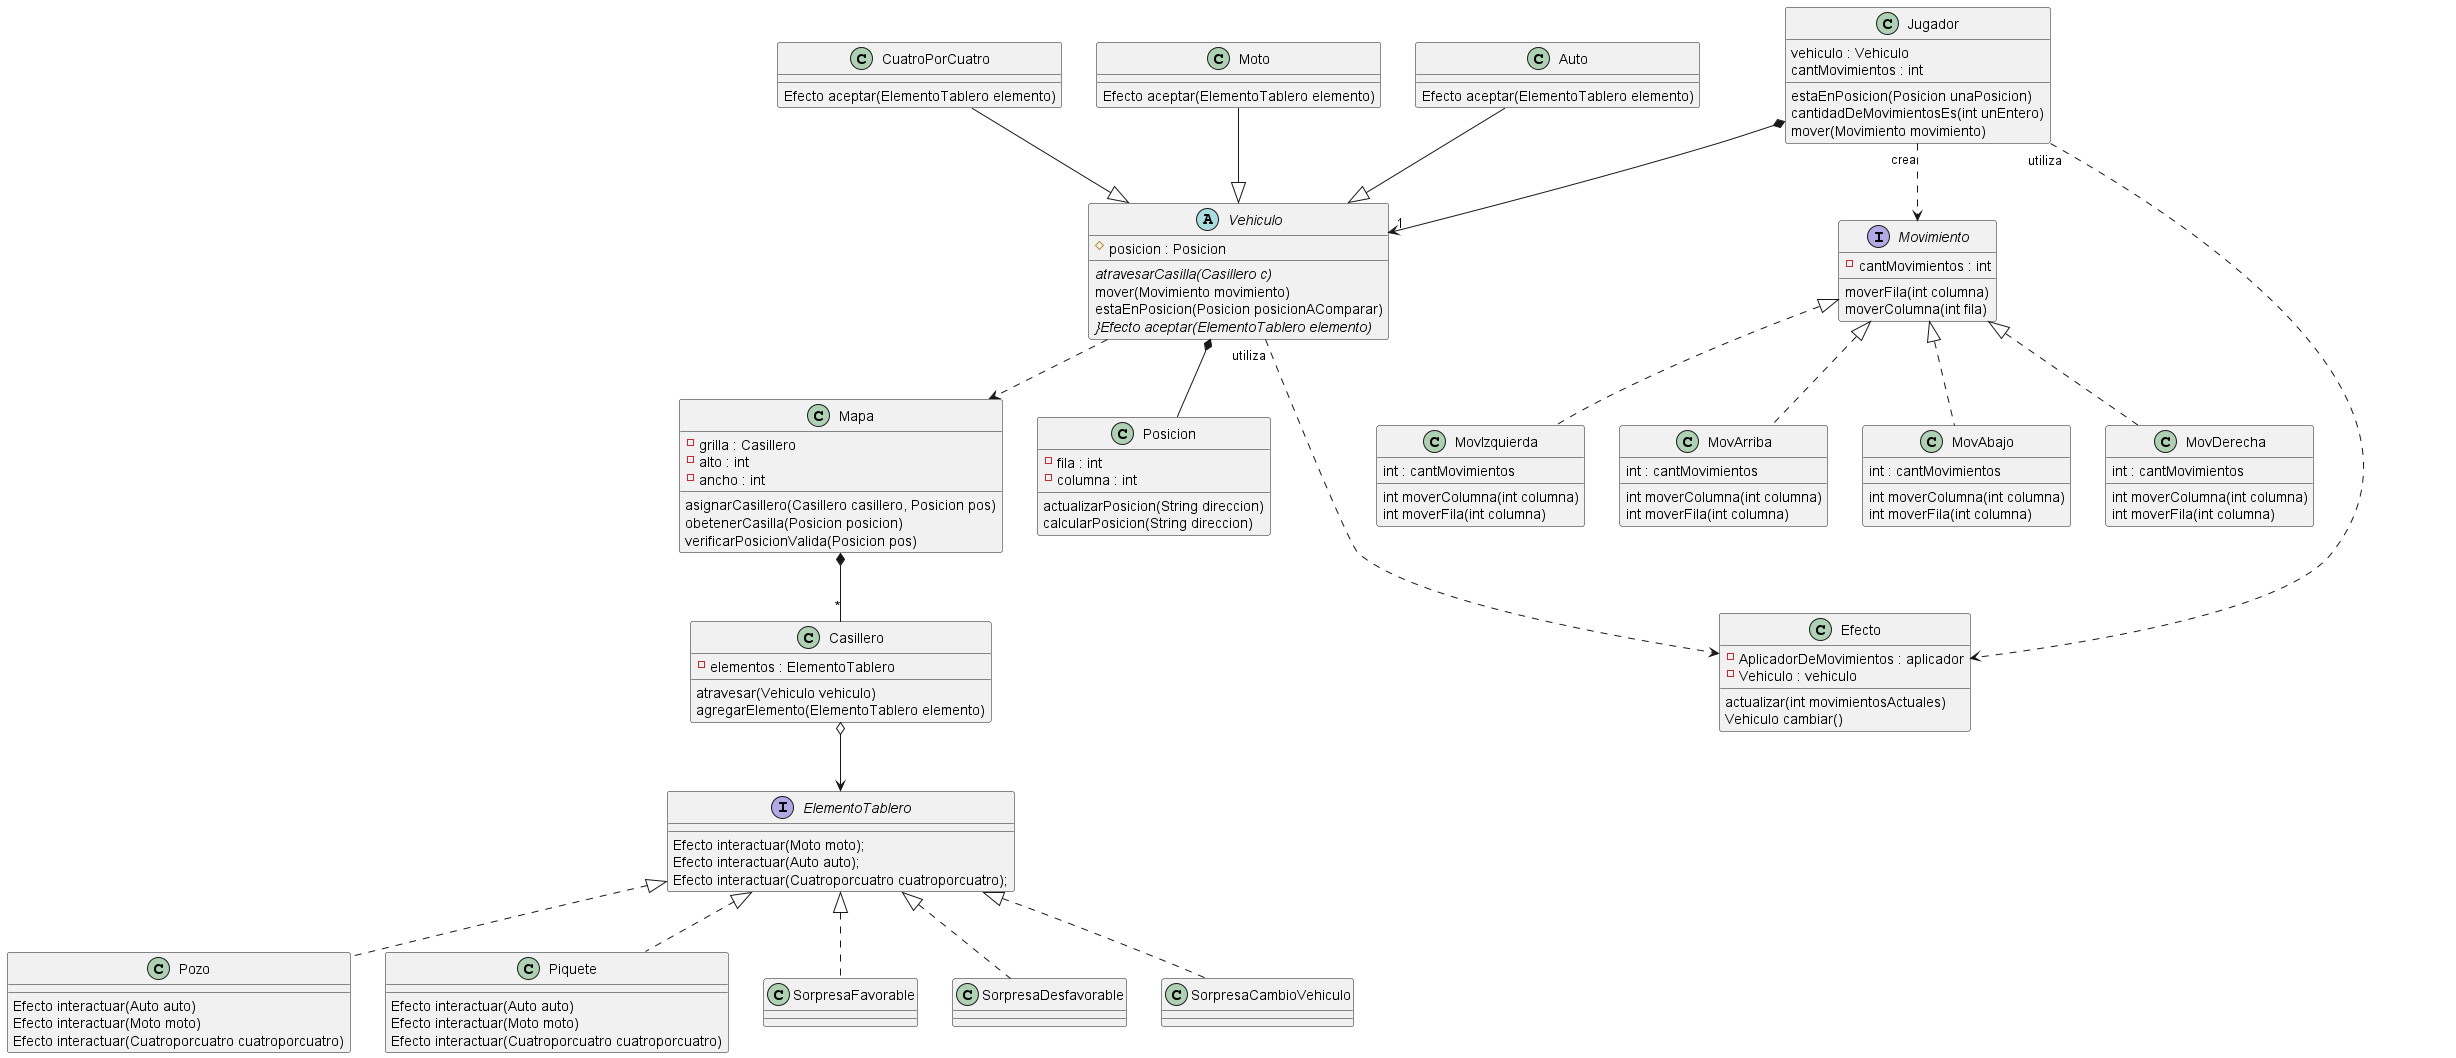
\includegraphics[width=1\textwidth]{diagrama de clase.png}
        \caption{\label{fig:class01}Diagrama del GPS-Challenge.}
    \end{figure}

    \section{Detalles de implementación}\label{sec:implementacion}
% Explicaciones sobre la implementación interna de algunas clases que consideren que puedan llegar a resultar interesantes.
    Para el diseño del mapa decidimos hacer uso de un HashMap el cual nos facilitará almacenar las casillas de todo el tablero. Para poder saber dónde guardarlo se hace uso de la función de Hash a la posición del casillero. De esta forma cuando queramos acceder a este casillero simplemente necesitaremos tener la posición.
    Aunque esto nos trae muchos beneficios también necesitamos saber cuándo el vehículo quiere moverse fuera del tablero para poder negarle esa acción. La forma en la que lo representamos fue asumiendo que sus dimensiones son cuadradas (es decir alto y ancho tienen el mismo valor). Nosotros pensamos el tablero con la posición (1,1) siendo la esquina superior izquierda y si se quiere mover el vehículo para abajo este debe cambiar su posición aumentándole uno a su fila quedando: (2, 1). Entonces a través de un método de mapa simplemente verifica si la posición en la que se quiere mover el vehículo esta dentro de las dimensiones del tablero.



    \section{Excepciones}\label{sec:excepciones}
% Explicación de cada una de las excepciones creadas y con qué fin fueron creadas.

    \begin{description}
        \item[Exception]
        \item[Excepcion]
        \item[Excepcion]
        \item[Excepcion]
        \item[Excepcion]
    \end{description}

    \section{Diagramas de secuencia}\label{sec:diagramasdesecuencia}
% Mostrar las secuencias interesantes que hayan implementado. Pueden agregar texto para explicar si algo no queda claro.



    \begin{figure}[H]
        \centering
        \includegraphics[width=1\textwidth]{secuencia moto.png}
        \caption{\label{fig:seq01}Secuencia de una moto moviéndose a través del mapa}
    \end{figure}



\end{document}
